
\section{Results}
Following the protocol outlined in section 3.2, we evolved 100 networks for each of the seven variants of the model. For all networks, we set network size to 2000 nodes; ; and . These choices are discussed in the appendix.

\subsection{Goodness-of-fit of the power-law model}

For each network evolved we computed two best-fit power-law models, one for formulaand the other for formulawhere formulais the in-degree the minimizes the Kolmogorov-Smirnov distance between the fitted function and the data over formula. On each of these models , we ran a goodness-of-fit test as described in section 3.2. This resulted in two distributions of p-values for our control group, plus two more for each of our six treatment groups. Table 3 and 4 report descriptive statistics for these distributions.

Table 3: Testing for goodness-of-fit of power-law models to degree distributions of interaction networks in online communities, with no onboarding and with onboarding. The parameter formulaapproximates the effectivess of the onboarding action. Power-law models are estimated over all nodes with degree formula.

From Table 3, we conclude that onboarding seems to have some effect on the goodness-of-fit of the generated data to their respective best-fit power-law models when formula. The effect goes in the direction of reducing the p-values. The rightmost column counts the networks for which the goodness-of-fit test returns a p-value below 0.1 (the threshold value below which the literature recommend Hypothesis 1 is rejected), out of the 100 runs. 

It is useful to address the question of whether Hypothesis 1 can be rejected in the aggregate, rather than for each individual network. We can do so by computing T-tests on the null hypothesis that the average p-value in each case is equal to 0.1, against an alternate hypothesis of p-value being smaller than 0.1. The results of such tests are summarized in Table 4.

Table 4: Testing for mean p-values equal to 0.01. The second column reports the value of the t statistic; the third column reports the probability of the alternate hypothesis mean < 0.1 being true. 0.1 is the threshold value below which our hypothesis H1 is rejected, as recommended by \cite{clauset2009power}. Power-law models are estimated over all nodes with in-degree formula.

Illustration 1 shows the cumulate density functions of the p-values in the control and treatment groups. 

Illustration 1: Cumulate Density Functions of p-values for each of the seven batches of networks. 20\% of the networks evolved without onboarding (dark blue) have degree distributions that test negatively for H1. When onboarding is introduced, that percentage rises to between 50 and 90%. A higher effectiveness of onboarding reduces the number of rejections. Power-law models are estimated over all nodes with degree formula.

When we consider only the upper tail of the in-degree distribution (formula), the effect of introducing onboarding on the goodness-of-fit is much less clear. All but 13 networks generated display scaling behavior in the upper tail when formula is chosen so as to minimize the Kolmogorov-Smirnov distance between the generated data and the best-fit power-law model. We conclude that we do not reject Hypothesis 2, regardless of whether onboarding is present or not. 

OLE-objectTable 5: Testing for goodness-of-fit of power-law models to in-degree distributions of interaction networks in online communities, with no onboarding and with onboarding. The  parameter approximates the effectivess of the onboarding action. Power-law models are estimated over all nodes with in-degree formula , where formula is the value that minimized the Kolmogorov-Smirnov distance between the fitted power-law model and the empirical data.

\subsection{Lower bounds}
Our results show a limited, albeit statistically significant, effect of onboarding on the value of formula, the value of formula that minimizes the Kolmogorov-Smirnov distance between the data generated by the computer simulation and the best-fit power-law model. Table 6 illustrates, for each batch of 100 networks, the average value of formula, its standard error and the  result of a t-test on the null hypothesis that formulavs the alternate hypothesis that formula, where denotes the effectiveness of the onboarding activity. 

OLE-objectTable 6: Testing the null hypothesis that formula Introducing onboarding has the effect to increase formula, the value that minimized the Kolmogorov-Smirnov distance between the fitted power-law model and the empirical data. This effect is statistically significant at the 5% level for , and at the 0.1% level for formula.

Illustration 2: Cumulate Density Functions of the degrees at which networks exhibit power law behaviour, for each of the seven batches of networks generated. A little over 60% of the networks evolved without onboarding (dark blue) approximate power-law models best when such power-law models are fitted with lower bound 3 or lower. When onboarding is introduced, that percentage decreases to between 20 and 50%.  

\begin{figure}[thb]
\centering

	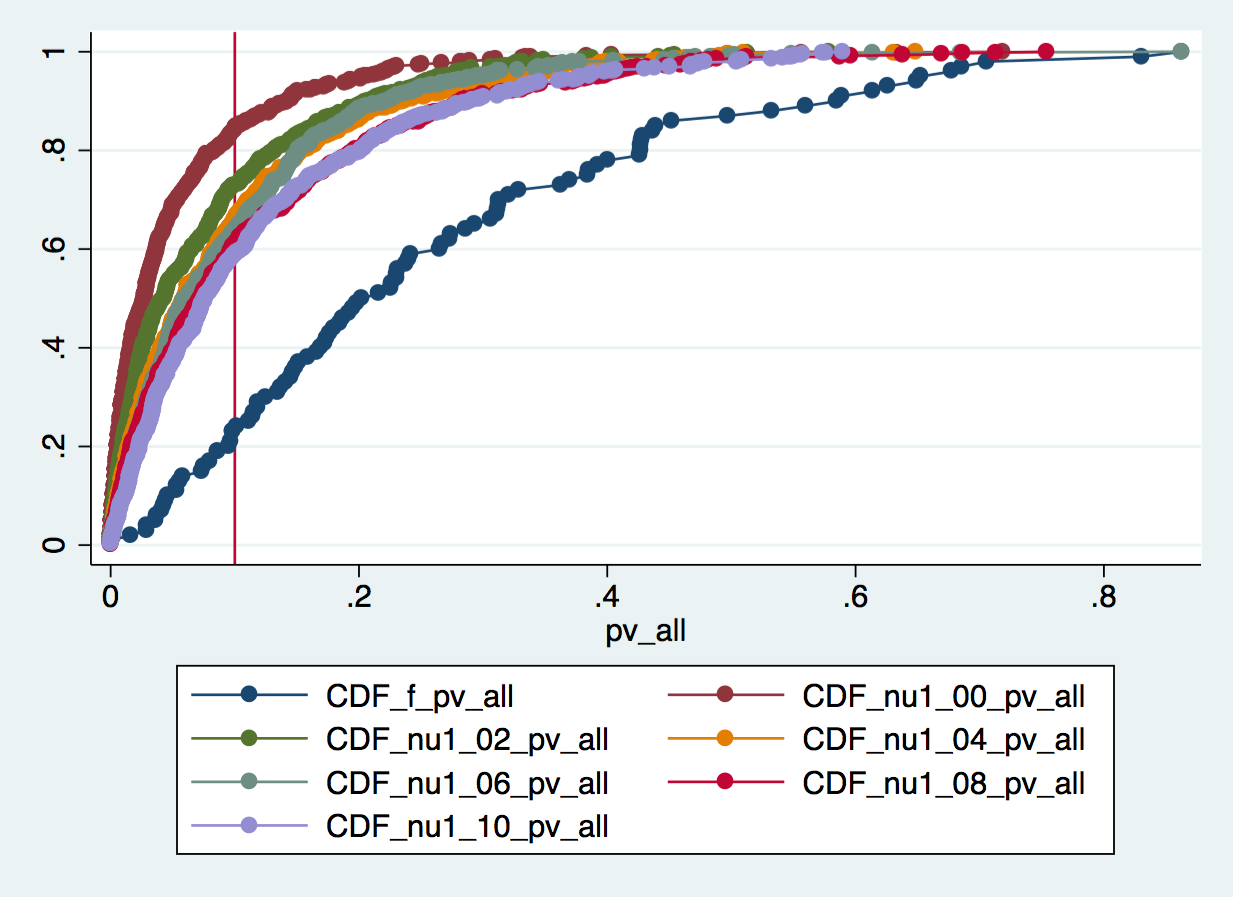
\includegraphics[width=.9\linewidth]{../Pictures/CDF_nu1.png}\label{fig:CDFnu1}
	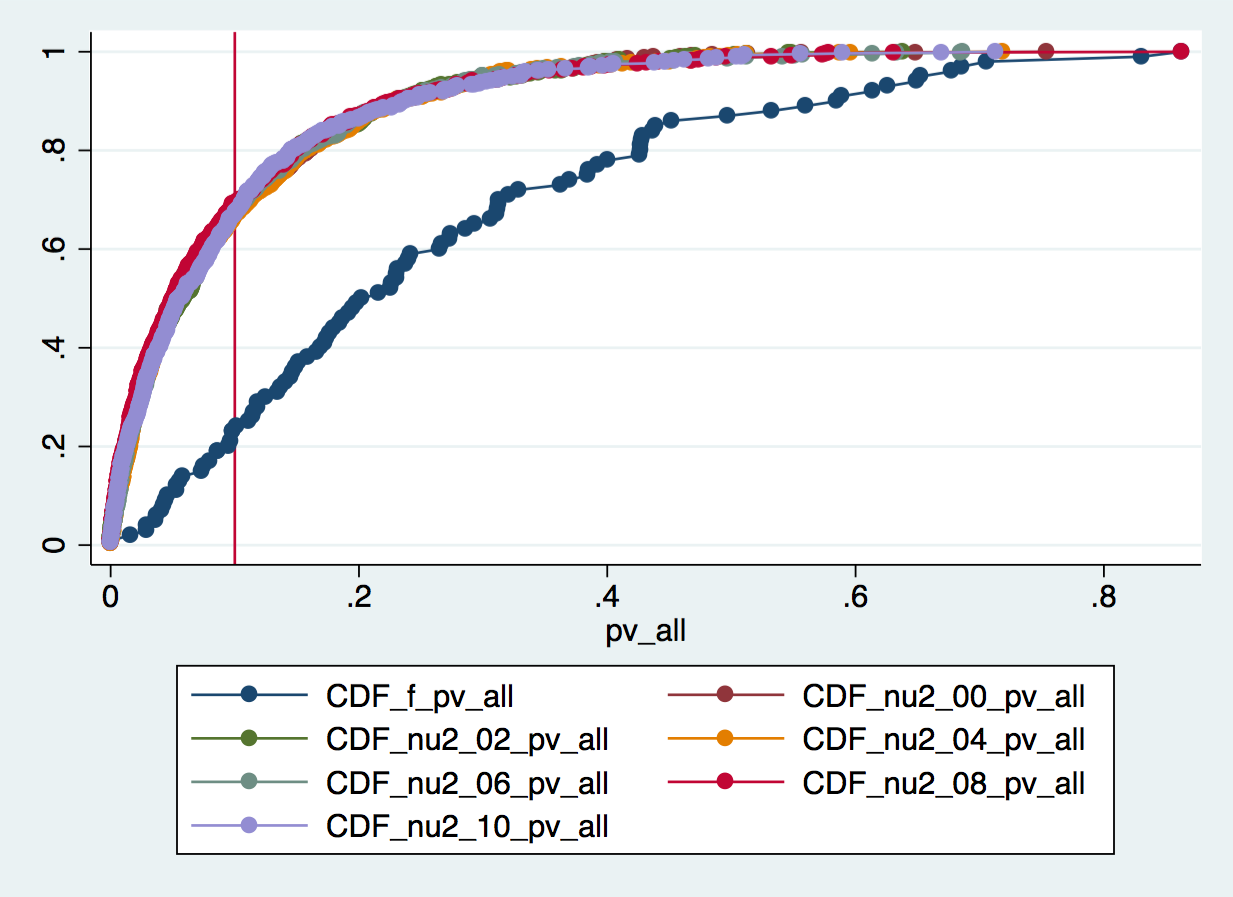
\includegraphics[width=.9\linewidth]{../Pictures/CDF_nu2.png}\label{fig:CDFnu2}
  %\subfloat[][]{}
  %\subfloat[][]{}
  \caption{Influence of parameters $\nu_1$ an $\nu_2$}
 \label{fig:CDF}
\end{figure}


\subsection{Exponents}
When considering only the tails of the in-degree distributions (formula), we find that introducing onboarding has a positive and significant on the value of the exponent. This is consistent with the theoretical results by Dorogovtsev and Mendes \cite{dorogovtsev2002evolution}, who proved that introducing a fraction of non-preferential attachment edges in evolving networks with preferential attachment does not suppress the power-law dependence of its degree distribution, but only increases the scaling exponent thereof. Table 7 summarizes the results of t-tests on the null hypothesis that formula against the alternative hypothesis that formula, where is the scaling exponent. 

OLE-objectTable 7: Testing the null hypothesis that   for different levels of onboarding effectiveness. When a p-value of 0.05 is set as the rejection threshold, the null hypothesis is rejected in favor of the alternative hypothesis that formulafor all values of the effectiveness parameter. When a p-value of 0.01 is chosen instead, the null hypothesis is rejected in favour of the alternative hypothesis in all cases, save for .